\documentclass{beamer}
\usetheme{Warsaw}
\useinnertheme{circles}
\useoutertheme[subsection=false]{smoothbars}
\usepackage[utf8x]{inputenc}
\usepackage[czech]{babel}
\usepackage[T1]{fontenc}
\usepackage{listings}
\usepackage{tikz}
\lstset{basicstyle=\tiny\ttfamily}
\logo{
\includegraphics[height=0.5cm]{brmlab.pdf}}

\begin{document}

\AtBeginSection[]
{
  \begin{frame}
    \frametitle{Outline}
    \tableofcontents[currentsection]
  \end{frame}
}

\title{brmiversity: Umělá inteligence \\ a teoretická informatika}
\subtitle{Přednáška č. 6}
\author{Petr Baudiš $\langle${\tt pasky@ucw.cz}$\rangle$}
\institute{
	brmlab 2011\\
	\vskip 1ex
	\pgfdeclareimage[height=4ex]{ccbysa}{by-sa.pdf}
	\pgfuseimage{ccbysa}
}
\date{}
\frame{\titlepage}

\section{Pravděpodobnost}

\subsection{}
\begin{frame}{Pravděpodobnost}
\begin{center}
Pravděpodobnost: Stane nebo nestane se nějaká náhodná událost?
\vskip 2ex
\begin{block}{Dvě interpretace}
\begin{itemize}
\item {\bf Subjektivisti:} Stav mysli, stupeň víry.
\item {\bf Frekventisti:} Konvergence série experimentů.
\end{itemize}
\end{block}
\vskip 2ex
({\bf Fuzzy logika} pracuje se stupni pravdivosti, to je něco jiného!)
\end{center}
\vskip 3ex
\begin{itemize}
\item Provádíme sérii {\em pokusů}, ty nám dávají {\em výsledky}, \\ množiny výsledků jsou {\em náhodné jevy}.
\end{itemize}
\end{frame}

\subsection{}
\begin{frame}{Matematická pravděpodobnost}
\begin{itemize}
\item Náhodný jev $A$ má pravděpodobnost $P(A) \in [0,1]$
\item Součet pravděpodobností všech základních jevů (jendotlivých výsledků) je 1; negace jevu je $1-p$
\item Jednoduchý případ --- rovnoměrně náhodný jev $A$ má po $n$ pokusech, z toho $m$ úspěšných, $P(A) \simeq m/n$
\vskip 3ex
\item Stane se $A$ nebo $B$? $P(A \cup B) = P(A) + P(B) - P(A \cap B)$
\item {\bf Nezávislé jevy} $A, B$ --- pravděpodobnost jednoho nezávisí na výskytu druhého
\item Stane se $A$ a $B$ zároveň? $P(A \cap B) = P(A) \cdot P(B)$, jsou-li nezávislé
\end{itemize}
\end{frame}

\subsection{}
\begin{frame}{Matematická pravděpodobnost}
\begin{itemize}
\item {\bf Podmíněná pravděpodobnost} --- jevy $A,B$ nejsou nezávislé
\item Stane se $A$ za předpokladu $B$? $P(A|B)$
\item $P(A \cap B) = P(A|B) \cdot P(B)$
\end{itemize}
\vskip 2ex
\begin{block}{Bayesova věta}
$$ P(A|B) = \frac{P(B|A)P(A)}{P(B)} $$
\end{block}
\vskip 3ex
\begin{itemize}
\item Diskrétní ``booleovský'' jev $A$ --- $P(A)$ že (ne)nastane
\item Spojitý jev $X$ --- interval čísel, očekávaná hodnota $\mathbb{E}[X]$
\end{itemize}
\end{frame}

\subsection{}
\begin{frame}{Statistika}
\begin{itemize}
\item Teorie pravděpodobnosti se zabývá abstraktními pravděpodobnostmi jevů
\item Statistika se zabývá pravděpodobnostmi, které jsme naměřili
\item {\bf Zákon velkých čísel:} Průměr (střední hodnota) naměřených hodnot konverguje k očekávané hodnotě
\vskip 3ex
\item Jak daleko jsou naměřené hodnoty od průměru?
\item {\bf Rozptyl} je střední kvadratická odchylka
\item {\bf Směrodatná odchylka} je odmocnina rozptylu
\end{itemize}
\end{frame}

\subsection{}
\begin{frame}{Pravděpodobnostní rozdělení}
\begin{columns}
\begin{column}{5.5cm}
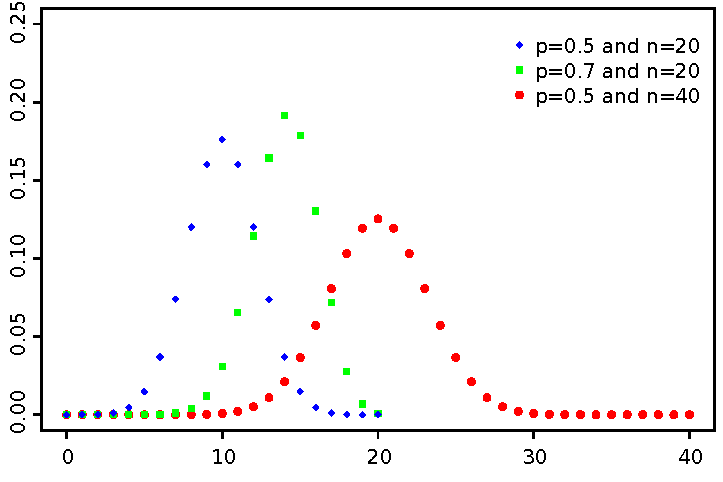
\includegraphics[width=5.5cm]{Binomial_distribution_pmf.pdf}
\end{column}
\begin{column}{5.5cm}
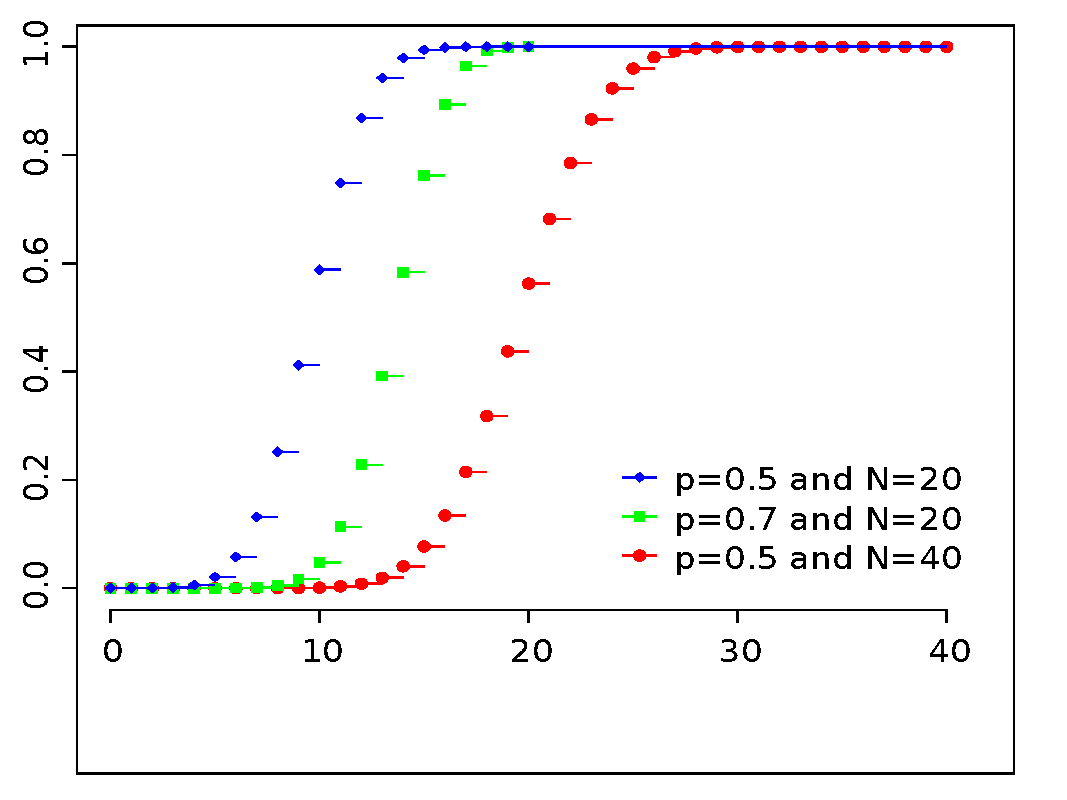
\includegraphics[width=5.5cm]{Binomial_distribution_cdf.pdf}
\end{column}
\end{columns}
\begin{itemize}
\item Pravděpodobnostní rozdělení popisuje pravděpodobnosti různých hodnot při určitém typu pokusu
\item Dává nám střední hodnotu a rozptyl \\ pro dané parametry pokusu
\item Bernoulliho rozdělení ($p$): Hod mincí
\item Binomiální rozdělení ($p,n$): Série Bernoulliho trialů
\item Poissonovo rozdělení ($\lambda,k$): Počet výskytů události za čas
\end{itemize}
\end{frame}

\subsection{}
\begin{frame}{Normální rozdělení}
\begin{columns}
	\begin{column}{5.5cm}
		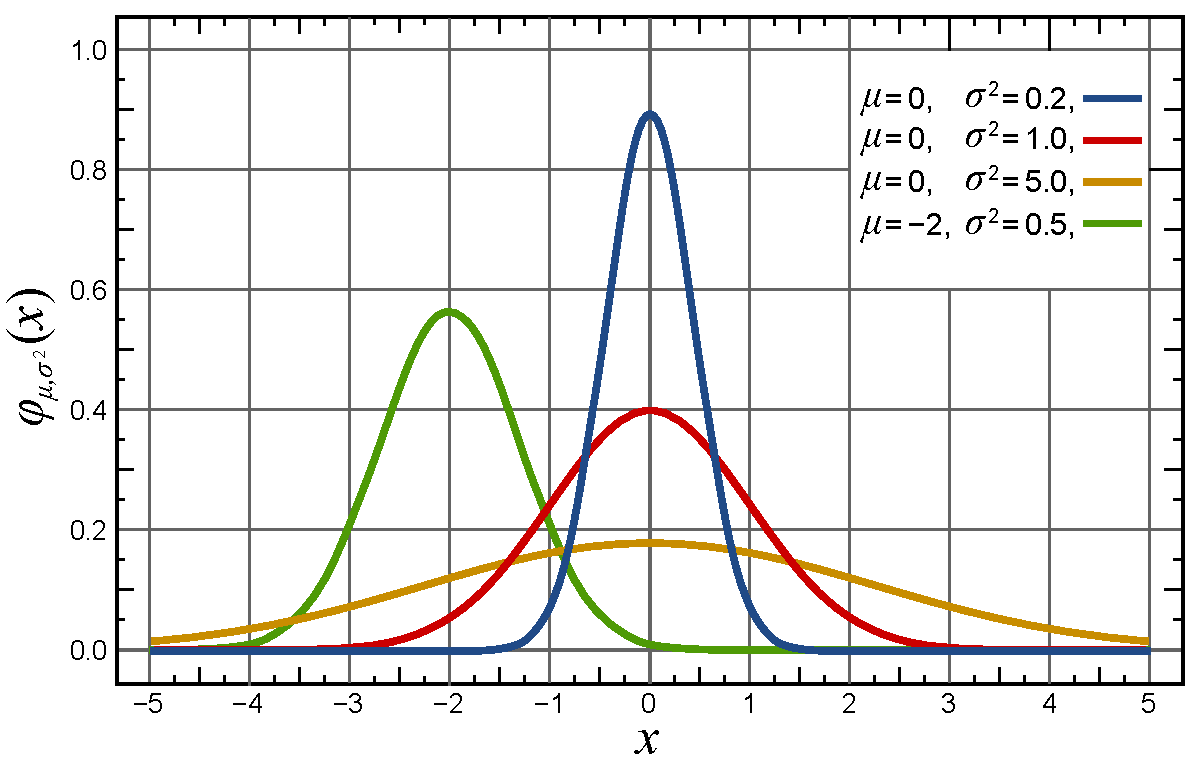
\includegraphics[width=5.5cm]{Normal_Distribution_PDF.pdf}
	\end{column}
	\begin{column}{5.5cm}
		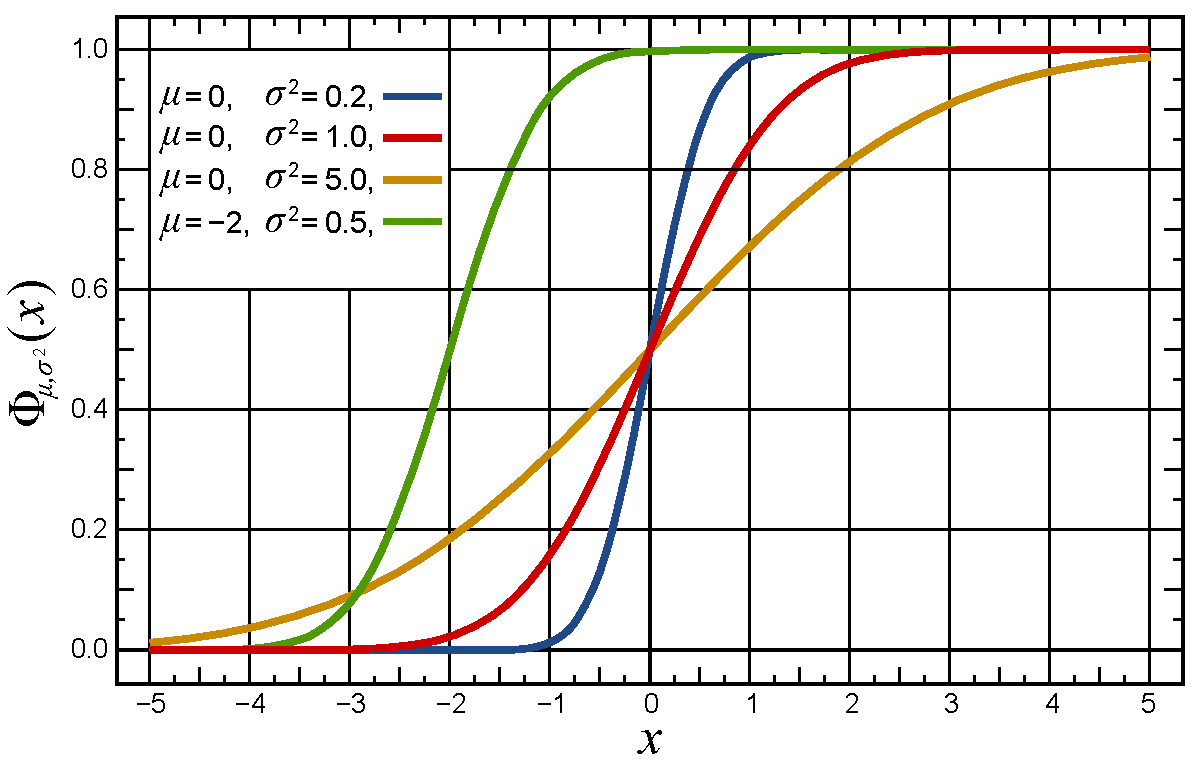
\includegraphics[width=5.5cm]{Normal_Distribution_CDF.pdf}
	\end{column}
\end{columns}

\begin{center}
Máme-li mnoho měření, konvergují k normálnímu rozdělení:
	$$ \frac{1}{\sqrt{2\pi \sigma^2}} e^{-\frac{(x-\mu)^2}{2 \sigma^2}} $$
\end{center}

\begin{itemize}
\item {\bf Interval spolehlivosti:} S pravděpodob. $p$ bude $\mathbb{E}[X] = \mu \pm \epsilon$
\item ``ODS by volilo $20\% \pm 3\%$ lidí'' --- s nějakou pravděpodobností (třeba $5\%$) by to bylo ještě více nebo méně
\item $95\%$ interval je $1.96\sigma$
\end{itemize}

\end{frame}

\section{Umělá inteligence}

\subsection{}
\begin{frame}{Zpracování neurčité informace}
\begin{itemize}
\item Data o světě jsou neurčitá
\item Úkony ve světě jsou neurčitá
\item \dots takže reálný svět je neurčitý
\item Neurčitost: Usuzování, rozhodování, modelování, učení
\end{itemize}
\end{frame}

\subsection{}
\begin{frame}{Bayesovské sítě}
\begin{itemize}
\item Chceme modelovat svět provázaných náhodných jevů
\item Bayesovská síť: Graf (DAG), uzly jsou jevy, hrany jsou podmíněné vazby
\vskip 3ex
\item Co se stane, když vidím tohle?
\item Co bych měl zjistit, abych si co nejvíce upřesnil obraz o světě?
\item Na čem nejvíce závisí, že se tohle stane?
\item Kvůli čemu se asi stalo tohle?
\end{itemize}
\end{frame}

\subsection{}
\begin{frame}{Pravděpodobnostní rozhodovací stromy}
\begin{itemize}
\item Chceme posoudit dopady svých rozhodnutí \\
	Posloupnost rozhodnutí a neurčitých jevů \\ vede k různému užitku
\item Rozhodovací stromy: Větvení na rozhodnutích a jevech, \\ list je užitek
\item (Pozor, ``rozhodovací stromy'' se říká i něčemu jinému!)
\vskip 3ex
\item Kterou cestou má jet robot?
\end{itemize}
\end{frame}

\subsection{}
\begin{frame}{Influenční diagramy}
\begin{itemize}
\item Podstromy rozhodovacích stromů se často opakují, \\ nezáleží na předchozích rozhodnutích a jevech
\item Influenční diagramy (rozhodovací grafy): \\ Obecný graf, užitkové uzly udávají změnu užitku, \\ když skrze ně projdeme
\end{itemize}
\end{frame}

\subsection{}
\begin{frame}{Otázky?}
\begin{center}
Příště UI: Modelování --- Markovské modely, Kalmanův filtr.
\end{center}
\end{frame}

\section{Složitost}

\subsection{}
\begin{frame}{Pravděpodobnostní algoritmy}
\begin{itemize}
\item Po algoritmu obvykle chceme, aby nám vrátil \\ přesný výsledek za přesný čas
\item Co když akceptujeme určitou {\em malou chybu}?
\item Co když akceptujeme, že {\em jen asi} doběhneme včas?
\vskip 3ex
\item Model: Probabilistický Turingův stroj
\end{itemize}
\end{frame}

\subsection{}
\begin{frame}{Monte Carlo}
\begin{columns}
\begin{column}{7cm}
\begin{itemize}
\item Monte Carlo algoritmus: \\ Čím déle běžíme, tím \\ přesnější výsledek dostaneme.
\item Třída složitosti BPP: Problém \\ řešitelný na probabilistickém TS \\ v polynomiálním čase \\ s pravděpodobností chyby $\le 1/3$
\vskip 3ex
\item Obsah průniku kružnic
\item Určitý integrál (plocha pod křivkou)
\item Prvočíselné testy
\item Monte Carlo Tree Search
\end{itemize}
\end{column}
\begin{column}{4cm}
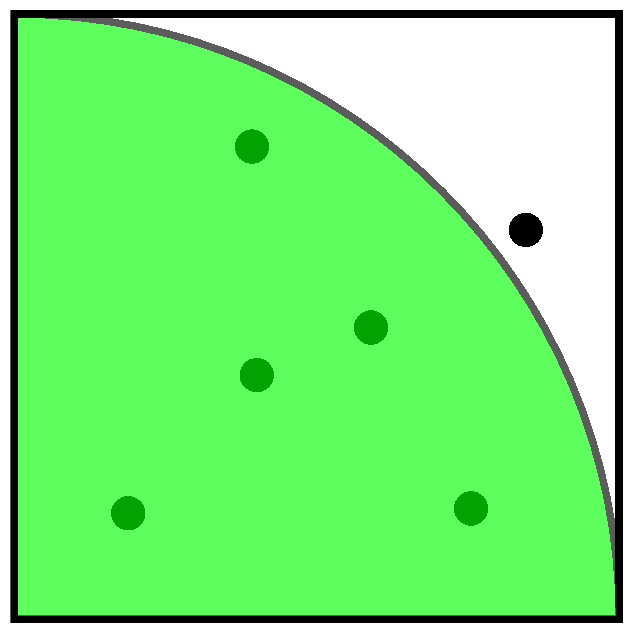
\includegraphics[width=4cm]{MC-pi.pdf}
\end{column}
\end{columns}
\end{frame}

\subsection{}
\begin{frame}{Las Vegas}
\begin{itemize}
\item Las Vegas algoritmus: {\em Očekávaná} doba běhu \\ je jiná než nejhorší
\item Třída složitosti ZPP: Problém řešitelný na \\ probabilistickém TS v očekávaném polynomiálním čase
\vskip 3ex
\item Quicksort s náhodnou volbou pivota
\vskip 3ex
\item Je Las Vegas a Monte Carlo ekvivalentní?
\end{itemize}
\end{frame}

\subsection{}
\begin{frame}{Otázky?}
\begin{center}
Příště: Míry složitosti, Savitchova věta, konstruovatelné funkce.
\end{center}
\end{frame}

\section{Datové struktury}

\subsection{}
\begin{frame}{Hashování}
\begin{itemize}
\item Hash tabulka (v paměti --- ``interní'').
\item Možná i nudle ven, řetězce.
\end{itemize}
\end{frame}

\subsection{}
\begin{frame}{Model hashování}
\begin{itemize}
\item Očekávaný počet kolizí, složitosti.
\end{itemize}
\end{frame}

\subsection{}
\begin{frame}{Externí hashování}
\begin{itemize}
\item Externí hashování.
\end{itemize}
\end{frame}

\subsection{}
\begin{frame}{Perfektní a univerzální hashování}
\begin{center}
Perfektní hashování: Chceme vyrobit \\ read-only hash tabulku bez kolizí.

\vskip 6ex

Univerzální hashování: Chceme vyrobit hashovací funkci \\ odolnou k nerovnoměrnému rozdělení vstupu.
\end{center}
\end{frame}

\subsection{}
\begin{frame}{Otázky?}
\begin{center}
Příště: Univerzální a perfektní hashování. \\ A někdy doděláme ty haldy.
\end{center}
\end{frame}

\subsection{}
\begin{frame}{Děkuji vám}
\begin{center}
{\bf pasky@ucw.cz}

\vskip 6ex

Příště: Umělá inteligence. \\ Neuronové sítě (statistické zpracování dat). \\ Adaptivní agenti (komunikace a znalosti). Datové struktury.
\end{center}
\end{frame}

\end{document}
